\chapter{Basics}

This chapter covers basics such as the analog to digital (A/D) conversion and the General Purpose Input/Output (GPIO).

\section{Analog to digital conversion}

In order to interact with the analog world, digital controllers possess two types of converters, which can be used as inputs (analog to digital) or outputs (digital to analog). The two major characteristics are the precision in bits and the sampling rate in $bits.s^{-1}$.
\\
\\
The digital to analog converter is very simple to build, with resistors placed alongside the bit lines. However, the analog to digital converter is much more complex and might use varying types of architectures (there exists a dozen of them). The AM3359 has an 8 channel, 12\,bits Successive Approximation (SAR) ADC, which means the input voltage is successively comparated to an internal voltage. Though it does not perform as well in general as a Wilkison ADC, it works better when the number of channel is high (in algorithmic terms, o(log(channels)) vs o(channels)). On the BeagleBone, there are 7 pins capable of doing A/D or D/A conversion with a precision of 12\,bits (error: 2.5 $10^{-4}$) and a sampling rate of 100\,000 samples per second. For comparison, the AVR Atmega32 has a precision of 10\,bits (error: 9 $10^{-4}$) and a sampling rate of around 10\,000 values (highly variable) per second. This is plenty enough to imagine making an oscilloscope with a decent resolution.
\\
\\
The A/D pins are used from the userpace via a virtual filesystem, under
\\
\verb!/sys/devices/platform/tsc/ainX!
\\
The A/D conversion is one of the most basic features expected from an embedded device for it allows to easily retrieve values from inert sensors which behave like variable resistances. Because the BeagleBone A/D pins do not tolerate more than 1.8\,V, the usual solution is to use a voltage divider with the grounded resistance being the sensor as desribed by figure~\ref{fig:voltagedivider}.
In some cases, a voltage divider cannot be used because the sensor does not output enough current to go through the divider. It is possible to use a pull-up resistor and a diode in order to not damage the lower voltage device, as desribed by figure~\ref{fig:pullupdiode}. When the 5\,V device is sending a logical ``0'', the whole line is pulled to 0. However, a logical ``1'' is going to be blocked by the diode, and therefore the 3.3\,V voltage applies on the other side of the diode.

\begin{figure}[ht]
%\centering
\subfigure[Voltage divider]{
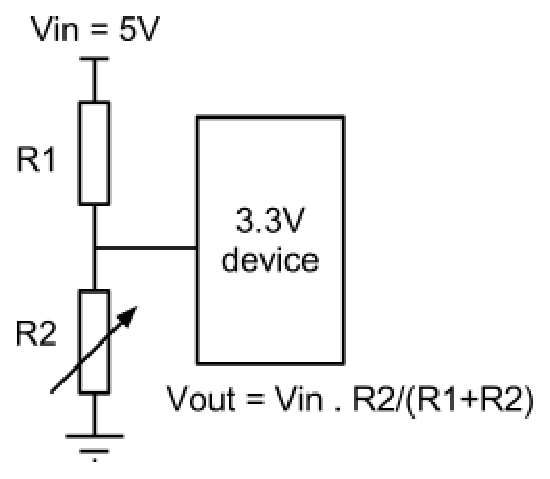
\includegraphics[width=5.5cm]{pictures/voltagedivider}
\label{fig:voltagedivider}
}
\subfigure[Simple 5V to 3.3V communication]{
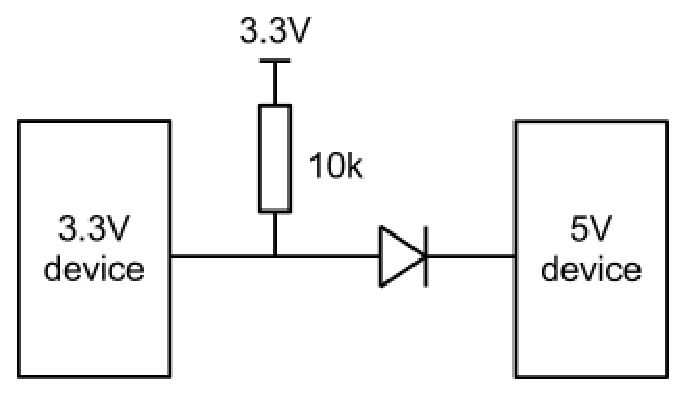
\includegraphics[width=7cm]{pictures/pullupdiode}
\label{fig:pullupdiode}
}
\end{figure}

%\begin{figure}[h!]
%\centering
%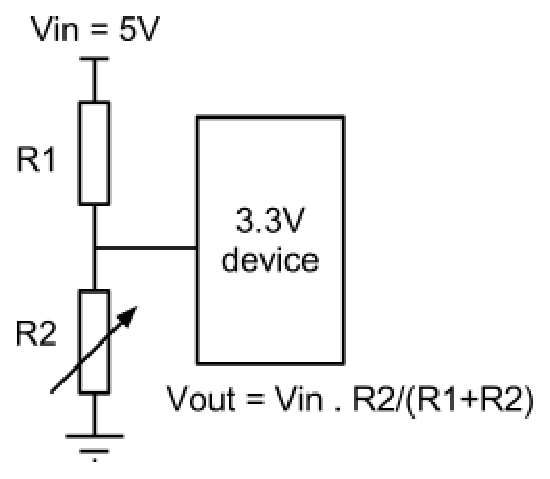
\includegraphics[width=6cm]{pictures/voltagedivider}
%\caption{Voltage divider}
%\label{fig:voltagedivider}
%\end{figure}

%\begin{figure}[h!]
%\centering
%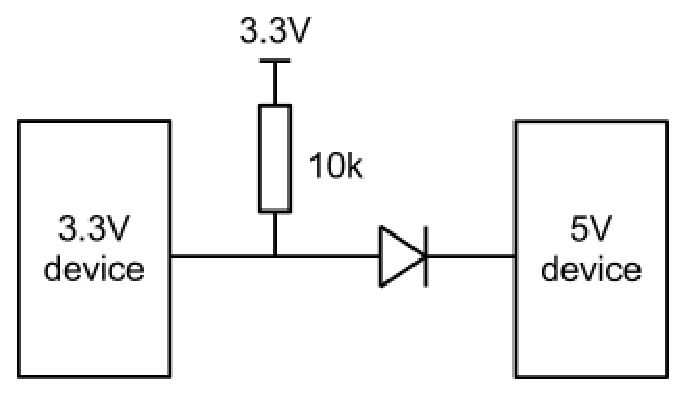
\includegraphics[width=7cm]{pictures/pullupdiode}
%\caption{Simple 5V to 3.3V communication}
%\label{fig:pullupdiode}
%\end{figure}

\section{General Purpose Input Output communication}

A GPIO is a digital hardware pin which can be controlled through the software. It can be used as an input or an output, and since it is digital, it uses the logic levels 0 and 1. Because chips have a limited number of pins (here, 66 on the headers), it sometimes happens that the pin to use necessitates a different MUX setting than the default \verb!MODE0!. The AM3359 has up to 8 different MUX modes per pin, and selecting one of them is going to route the pin to the desired internal logics of the chip. Some pins have no mux modes, such as the A/D pins.
\\
\\
A major evolution of the BeagleBone compared to the BeagleBoard, is that the GPIO pins are directly controllable through software, and that a virtual filesystem can be used to interact with them. Also, one can freely reconfigure the MUX pins. This means that it is not necessary to recompile the kernel when  a MUX value is changed! Then, the usual parameters are the enabling of the GPIO pin, its direction (in/out) and its value to read or write.
\\
\\
The MUX value of a pin is changed under \verb!/sys/kernel/debug/omap_mux!
\\
The rest of the GPIO control is under \verb!/sys/class/gpio/gpioX/!
\\
\\
Below is an example of using a GPIO pin in shell script, a command-line user interface interpreted language. Let us suppose that, for practical reasons, we want to use the first pin available on the P9 header. By looking at the datasheet, we can tell its name is \verb!UART4_RXD!. This means that if we intend to use this pin as a GPIO pin, the MUX has to be set first (mode 7), to configure the pin as \verb!gpio0[30]!. In order to change the MUX setting, we need to retrieve the actual name of the pin as far as the kernel is concerned. The \verb!MODE0! of our pin is named \verb!gpmc_wait0!, so we need to find a file with this name in the \verb!omap_mux! folder.
\\
\begin{lstlisting}[language=sh, basicstyle=\scriptsize]
#/bin/sh

echo 30 > /sys/class/gpio/export                #export the pin, it is now usable
echo 7 > /sys/kernel.debug/omap_mux/gpmc_wait0  #change the MUX setting to 7 (gpio mode)
echo out > /sys/class/gpio/gpio30/direction     #change the direction of the pin
echo 1 > /sys/class/gpio/gpio30/value           #write logical "1" to the pin!
echo 30 > /sys/class/gpio/unexport              #unexport the pin for a clean exit
\end{lstlisting}

Note that this method is the simplest, but also the slowest. If the speed at which the toggle can occur, and its preciseness in time are higher, two options are available:
\begin{itemize}
\item Direct register access: by mapping into memory the registers (as described in the PWM chapter), the actual delays of context switching from userspace to kernel space is bypassed, but there is an extensive documentation work to make to find register addresses (see AM335x technical reference manual \cite{amtrm})
\item PRU: the Programmable Real-time Unit is a dedicated unit capable of real-time in the AM3359 chip. It is a very complicated and time intensive solution, but it yields the best results.
\end{itemize}

Some interesting features of the GPIO pins is that, depending on their setting, they can be used to generate PWM output, for TTL communication such as I$^{2}$C or SPI and UARTs, or to set timers and interrupts.

\section{Communication protocols}

A UART is an asynchronous configurable hardware device usually used for serial communcation. Its goal is to translate bytes into series of bits and inversely, to minimize the number of wires used. It is associated with a protocol, such as RS-232.
\\
\\
SPI is a synchronous serial data link, developed by Motorola. It is based on a master/slave architecture, in full duplex mode. It uses 4 wires: a serial clock, a master output (resp. slave input) and a master input (resp. slave output), and a slave select.
\\
\\
I$^{2}$C is a serial bus, developed by Philips. It uses a multi-master/slave architecture, with 2 wires only: a serial clock and a data line. 
SPI has a higher throughput than I$^{2}$C, and consumes less power since it does not use pull-up resistors. On the other hand, I$^{2}$C uses fewer lines, is easier to debug and is more adapted to multinode communciation. A lot of electronic module boards embedding dedicated chips typically use SPI/I$^{2}$C.
\\
\\
Note that a level-shifter (3.3/5\,V) is usually necessary for I$^{2}$C, since the data line is bidirectional. With SPI, it is possible to implement electronics to avoid using a level-shifter, but it is recommended nonetheless.
